\section{Diseño del Prototipo }

Se hace mencion que apesar que la documentacion para elaborar el software esta en español, es un estandar el escribir codigo en ingles por tanto para mantener coherencia los diagramas mostrados a continuacion se usara este idioma para los nombres de las variables, funciones y clases.
\subsection{Definición de Requisitos:  }
    
\begin{enumerate}
    \item \textbf{Datos sobre infracciones de tráfico:} La captura de datos detallados sobre infracciones de tráfico, como la hora de la infracción, las coordenadas GPS, el tipo de infracción, los datos de identificación del vehículo e imágenes o vídeos, garantiza que cada incidente se documenta exhaustivamente. Este registro exhaustivo proporciona transparencia y responsabilidad, ya que los datos son inmutables y a prueba de manipulaciones una vez almacenados en la cadena de bloques. La inclusión de pruebas mediáticas refuerza aún más la credibilidad y verificabilidad de cada infracción, haciendo que los registros sean sólidos a efectos legales y administrativos. 
    \item \textbf{Información sobre el conductor:} Asociar las infracciones de tráfico a conductores concretos utilizando su dirección Ethereum (clave pública), los datos KYC si es necesario, y los números de identificación del conductor permite un seguimiento y una rendición de cuentas precisos. Esta vinculación permite al sistema personalizar el seguimiento y la verificación de las sanciones, garantizando que las sanciones se atribuyan correctamente a las personas adecuadas. El uso de datos KYC garantiza que las identidades de los conductores puedan verificarse de forma fiable, lo que resulta esencial para mantener la integridad y fiabilidad del sistema.
    \item \textbf{Datos de la sanción: }  Registrando los datos de la sanción, incluyendo el tipo de sanción, el importe de la sanción y el estado del pago de la sanción facilita la ejecución automatizada de las sanciones a través de contratos inteligentes. Esta automatización reduce la carga administrativa de y garantiza que las sanciones se apliquen de forma coherente y transparente. El registro inmutable de las sanciones y su estado de pago en la blockchain garantiza que el proceso sea justo y responsable, proporcionando una pista de auditoría clara para todas las transacciones financieras relacionadas con las infracciones de tráfico.
        \item \textbf{Eventos de contratos inteligentes:} El registro de eventos de contratos inteligentes, como el registro de nuevas infracciones de tráfico o la ejecución de sanciones, con datos relevantes y marcas de tiempo, garantiza que todas las acciones significativas se documenten de forma transparente. Este registro de eventos mejora la trazabilidad y la rendición de cuentas, proporcionando un registro cronológico de las actividades importantes del sistema. Esta transparencia es crucial para las auditorías y revisiones, ya que ayuda a generar confianza en las operaciones del sistema. 
        \item \textbf{Datos de las transacciones de la cadena de bloques: } El seguimiento de los datos de las transacciones de la cadena de bloques, incluido el hash de la transacción, las direcciones del remitente/receptor y las tarifas del gas, proporciona un registro detallado de todas las interacciones dentro del sistema. Estos datos permiten supervisar y auditar las transacciones, garantizando la transparencia y la trazabilidad. Además, hacer un seguimiento de las tarifas de gas ayuda a gestionar y optimizar los costes asociados a la ejecución de transacciones en la blockchain, que es importante para mantener la rentabilidad del sistema. 
        \item \textbf{Dispositivos de datos IoT:} La integración de datos de dispositivos IoT, como sensores o cámaras, junto con marcas de tiempo e identificación del dispositivo, puede mejorar las pruebas recopiladas para infracciones de tráfico. Estos datos en tiempo real proporcionan contexto adicional y pruebas corroborativas, haciendo que los registros de infracciones sean más sólidos y fiables. El uso de dispositivos IoT también puede automatizar la detección y el registro de infracciones, aumentando la eficiencia y la precisión del sistema.
            \item \textbf{Opiniones de los usuarios: } La recopilación de opiniones de los usuarios, incluidos el tipo de opinión, los comentarios y las valoraciones de los usuarios, ayuda a los administradores del sistema a comprender las experiencias y percepciones de los usuarios. Esta información es valiosa para identificar áreas de mejora en y mejorar la usabilidad y funcionalidad del sistema. Involucrar a los usuarios de esta manera puede conducir a un diseño del sistema más centrado en el usuario, mejorando la satisfacción y la eficacia general. 
                \item \textbf{Datos de cumplimiento: } El registro de los datos de cumplimiento, incluido el estado de cumplimiento y los detalles normativos, garantiza que el sistema se adhiere a las leyes y normativas de tráfico locales. Este seguimiento es vital para demostrar el cumplimiento de la normativa y evitar problemas legales. El mantenimiento de registros de cumplimiento detallados también facilita las auditorías reglamentarias en, proporcionando pruebas transparentes de que el sistema funciona dentro de las normas legales, lo que es esencial para generar confianza y credibilidad entre las partes interesadas.
\end{enumerate}

\subsection{Diagrama de casos de uso del sistema de gestión de infracciones de transito }
% img
\begin{figure}[htbp]
    \centering
    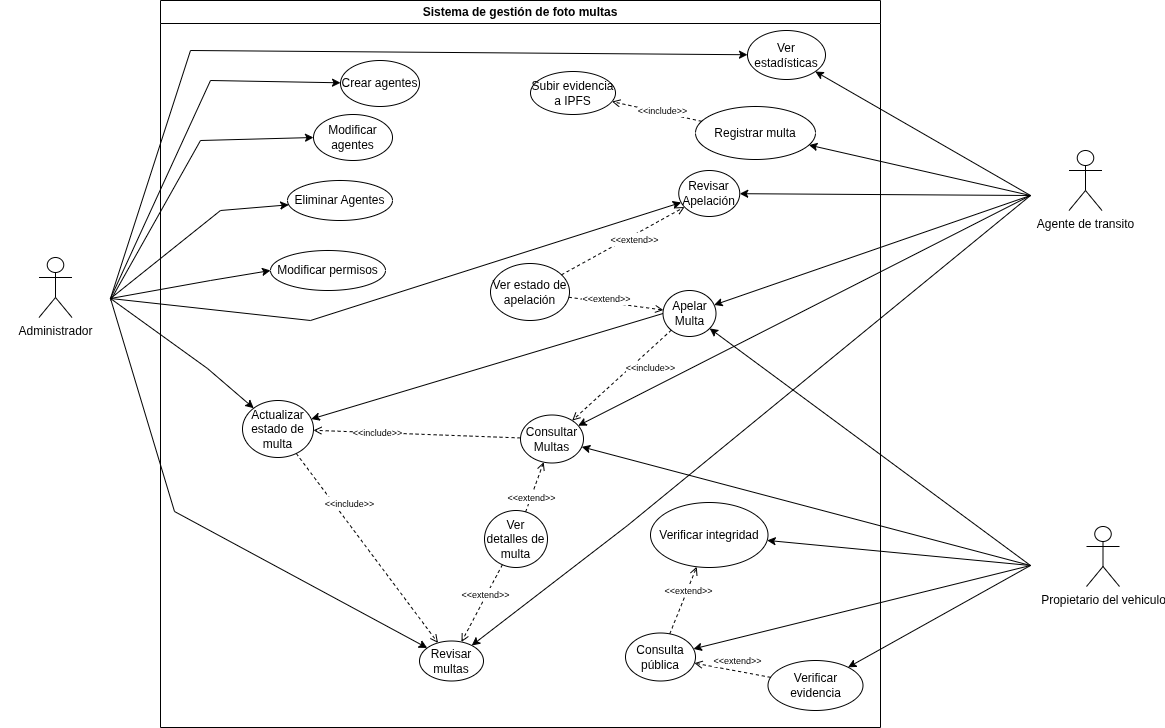
\includegraphics[width=0.8\textwidth]{Images/CasosUso.png}
    \caption{Diagrama de casos de uso del sistema de gestión de infracciones de tránsito.}
    \label{fig:casos_uso}
\end{figure}

 \subsection{ Diagrama de Despliegue }
\begin{figure}[htbp]
    \centering
    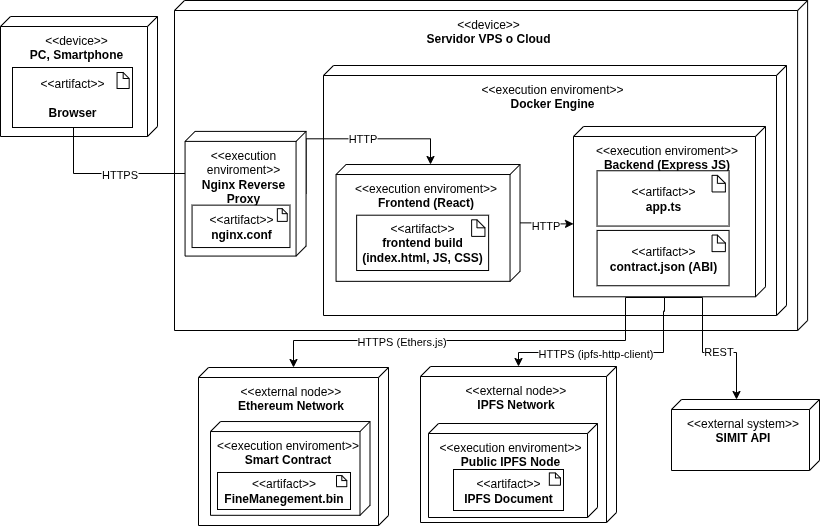
\includegraphics[width=0.8\textwidth]{Images/Despliegue.png}
    \caption{Diagrama de despliegue de la arquitectura del sistema.}
    \label{fig:diagrama_despliegue}
\end{figure}
En la Figura \ref{fig:diagrama_despliegue} se puede observar el diagrama de despliegue propuesto, donde cada nodo cuenta con la misma información, ya que esta se encontrará sincronizada. Asimismo, se conecta mediante servicios web a la base de datos de Apitude como herramienta de terceros para acceder a la información existente en el Registro Único Nacional de Tránsito (RUNT), de donde se obtendrán los datos de conductores, vehículos y el registro de infractores en Bogotá, así como el estado de las multas.

Hay que mencionar que existen dos soluciones para traer la información necesaria de estas entidades: la primera es una API llamada Apitude, de un tercero que provee la información del RUNT y del SIMIT; la segunda consiste en utilizar los datos que estas entidades públicas ya poseen en bases de datos tradicionales. 
 \subsection{ Diagrama de clases }
Hay que considerar que se manejarán dos capas de lógica: la primera enfocada en registrar los cambios en los estados de las multas a través de blockchain y la segunda capa encargada de la administración general de las multas (manipular los datos que no son visibles al público). 
 \begin{figure}[htbp]
    \centering
    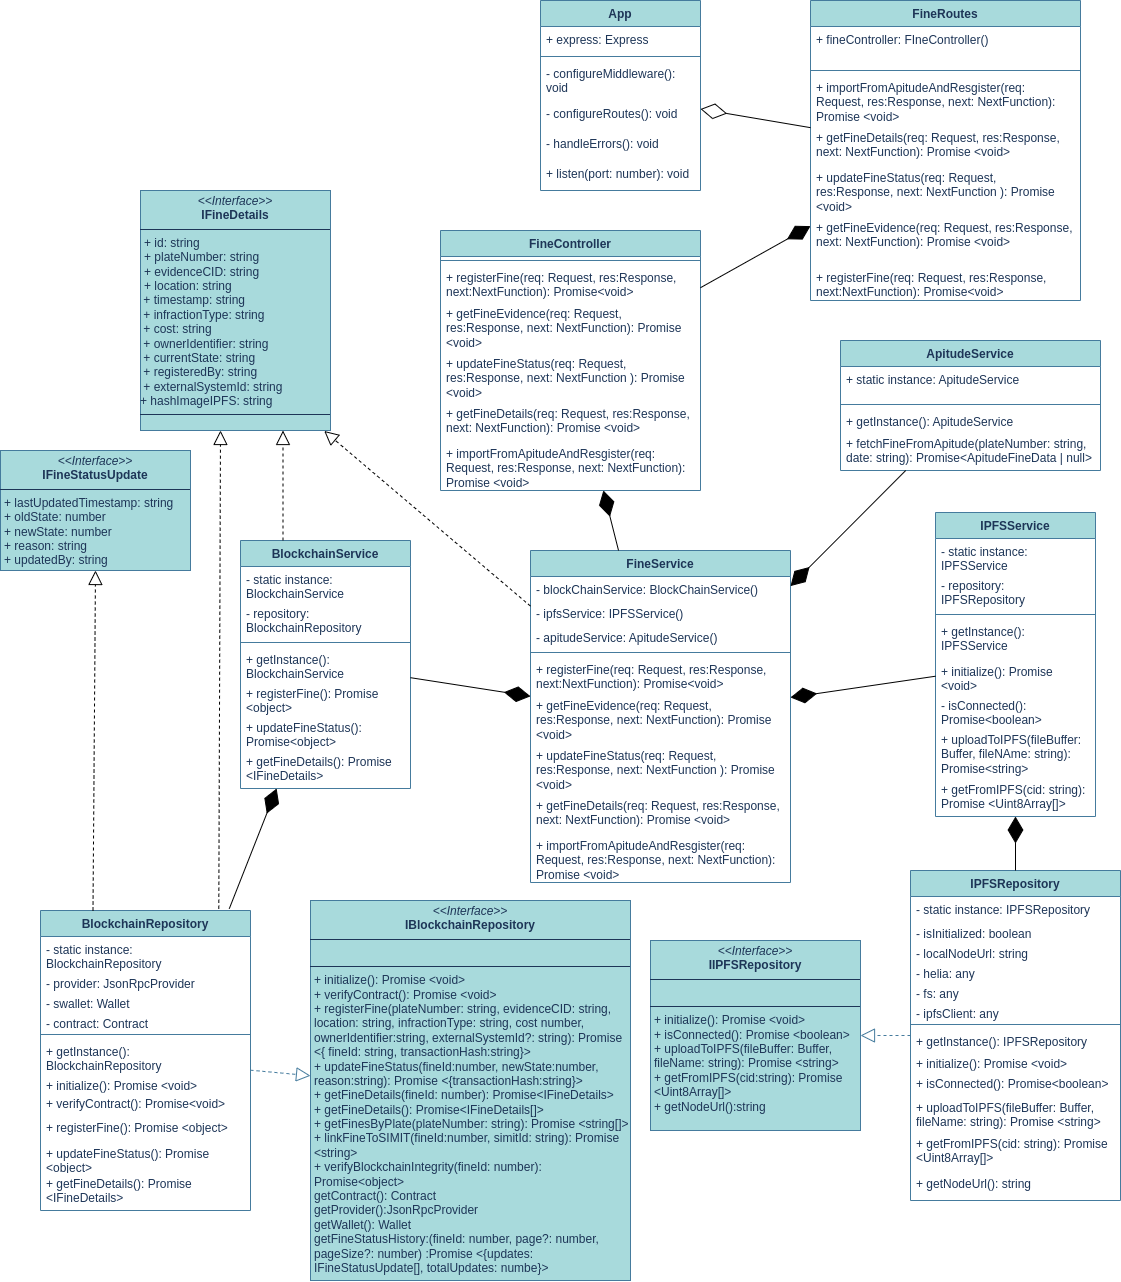
\includegraphics[width=0.8\textwidth]{Images/uml.png}
    \caption{Diagrama de clases del sistema de gestión de multas.}
    \label{fig:diagrama_clases}
\end{figure}
En la Figura \ref{fig:diagrama_clases} se hace un esquema de la primera capa lógica que se encarga de la administración general de las multas y los datos que maneja
 \begin{figure}[htbp]
    \centering
    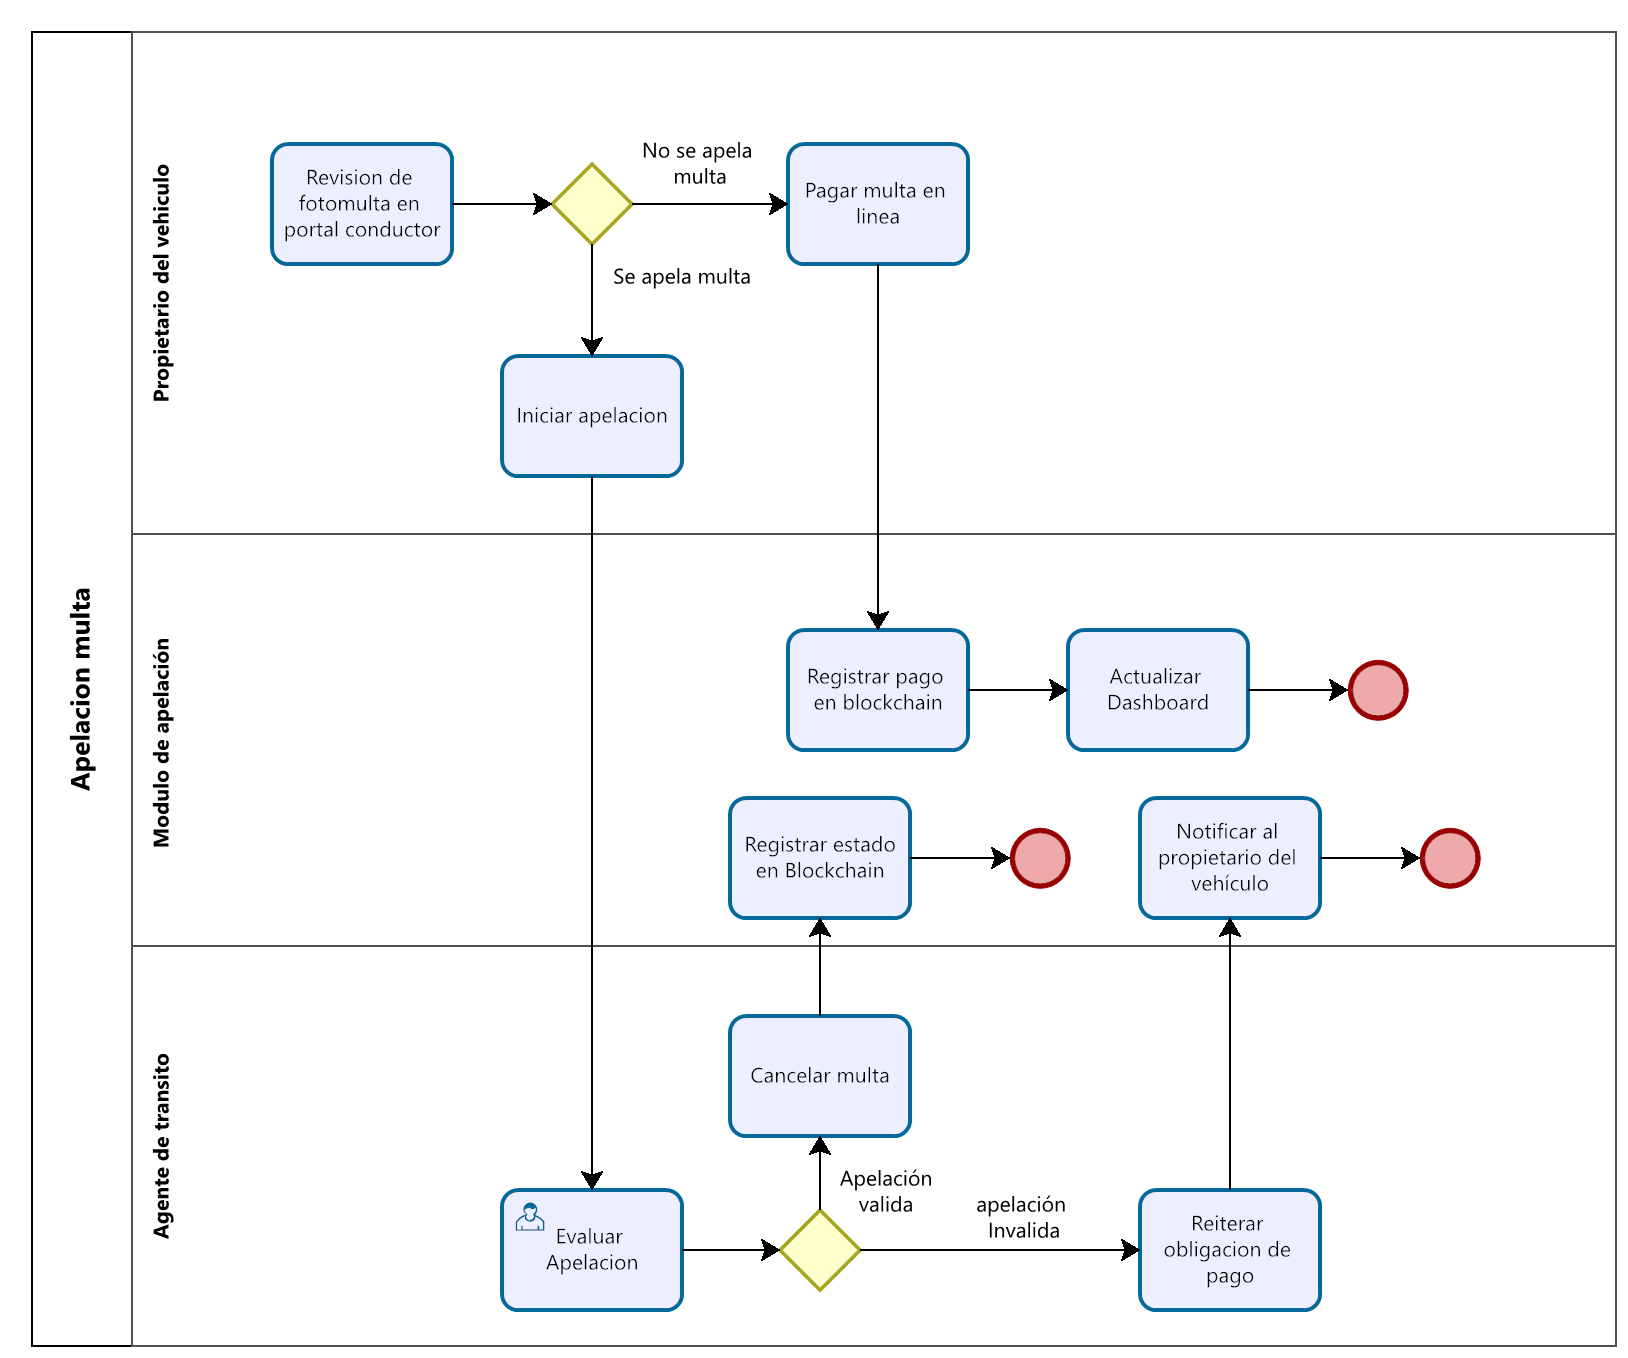
\includegraphics[width=0.8\textwidth]{Images/ActApelacion.png}
    \caption{Diagrama de actividades para el proceso de apelación de multa.}
    \label{fig:diagrama_apelacion}
\end{figure}
En la Figura \ref{fig:diagrama_apelacion} se hace mención en la segunda capa lógica la cual son los cambios generados en el registro de multas que registramos en la blockchain, que se traducen en los contratos realizados en solidity.
\subsection{ Diagrama de actividades }
 \begin{figure}[htbp]
    \centering
    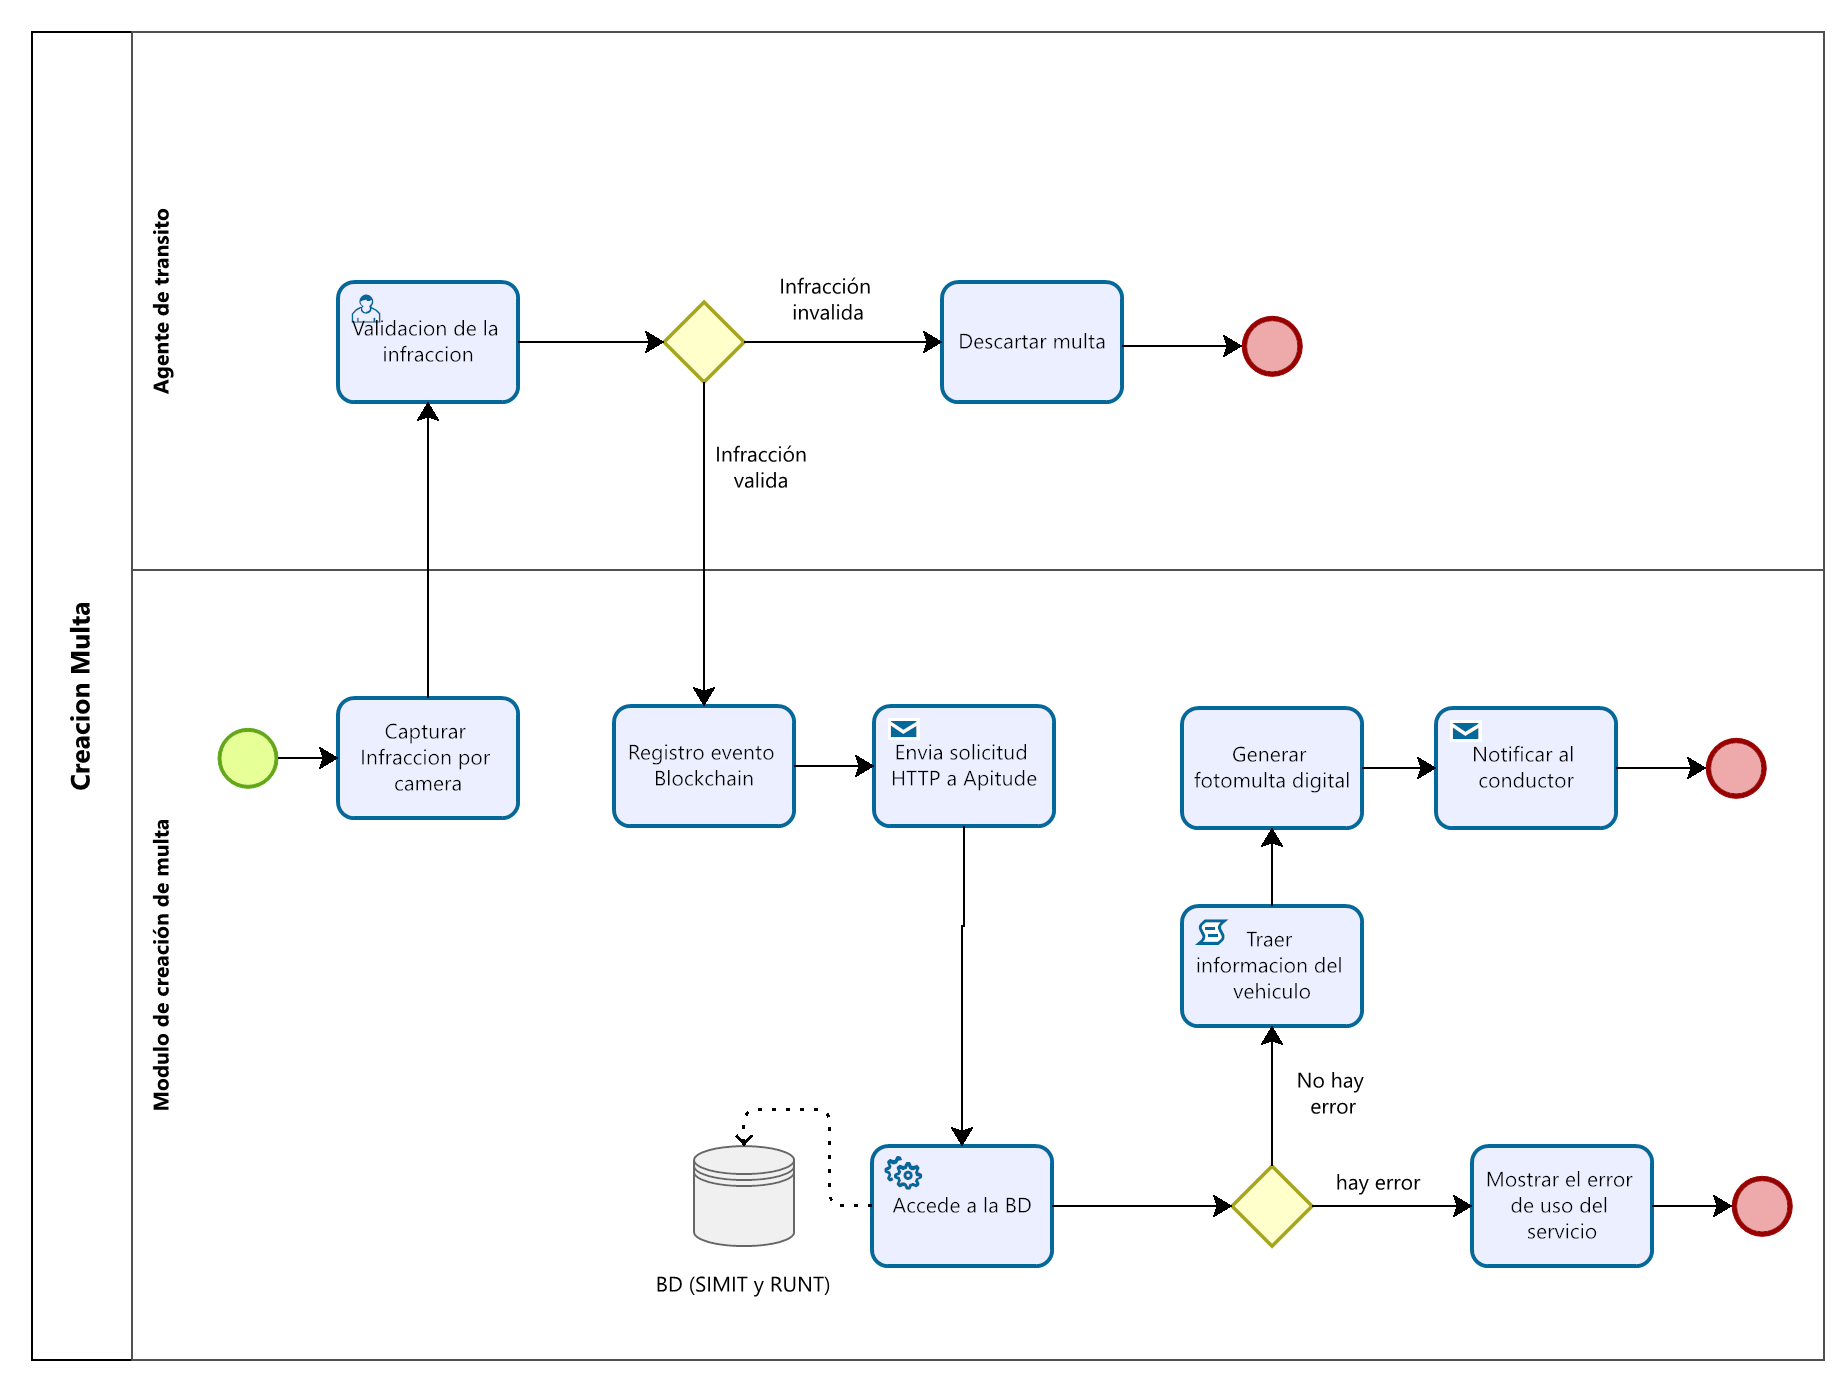
\includegraphics[width=0.8\textwidth]{Images/ActMulta.png}
    \caption{Diagrama de actividades para el proceso de creación de multa.}
    \label{fig:diagrama_creacion_multa}
\end{figure}
 \begin{figure}[htbp]
    \centering
    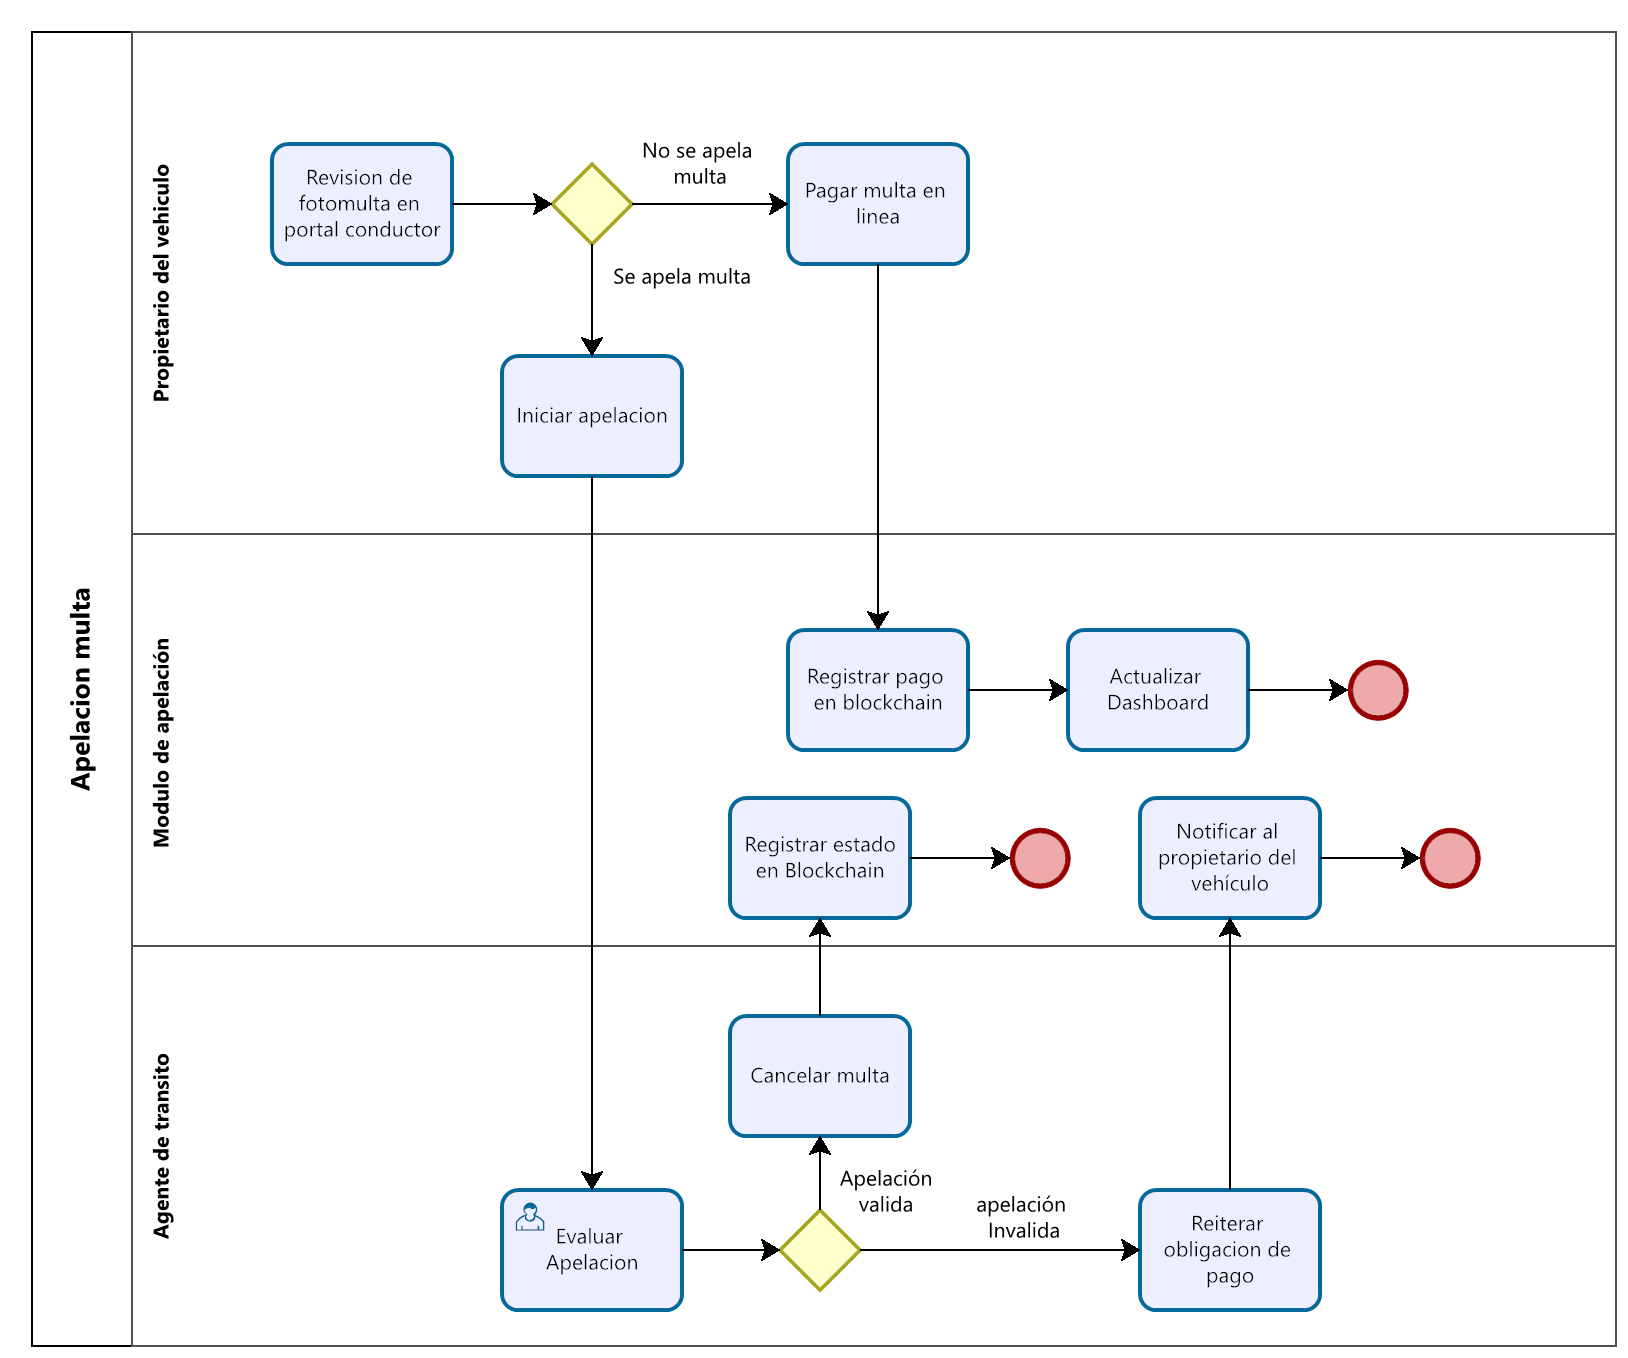
\includegraphics[width=0.8\textwidth]{Images/ActApelacion.png}
    \caption{Diagrama de actividades para el proceso de apelación de multa.}
    \label{fig:diagrama_apelacion_2}
\end{figure}

\subsection{Interfaz de Usuario}
\paragraph{Compartidas}
 \begin{figure}[htbp]
    \centering
    
\includegraphics[width=0.8\textwidth]{Images/UI1.png}
    \caption{Pantalla de login del sistema.}
    \label{fig:login}
\end{figure}
+En la Figura~\ref{fig:login} se aprecia la pantalla de inicio de sesión, punto de entrada para todos los usuarios autorizados del sistema.

 \begin{figure}[htbp]
    \centering
    
\includegraphics[width=0.8\textwidth]{Images/UI2.png}
    \caption{Pantalla de recuperación de contraseña.}
    \label{fig:recuperar_password}
\end{figure}
+La Figura~\ref{fig:recuperar_password} muestra el formulario para recuperar la contraseña, reforzando la experiencia de autoservicio y seguridad de la plataforma.
\paragraph{Vista Agente}
\begin{figure}[htbp]
    \centering
    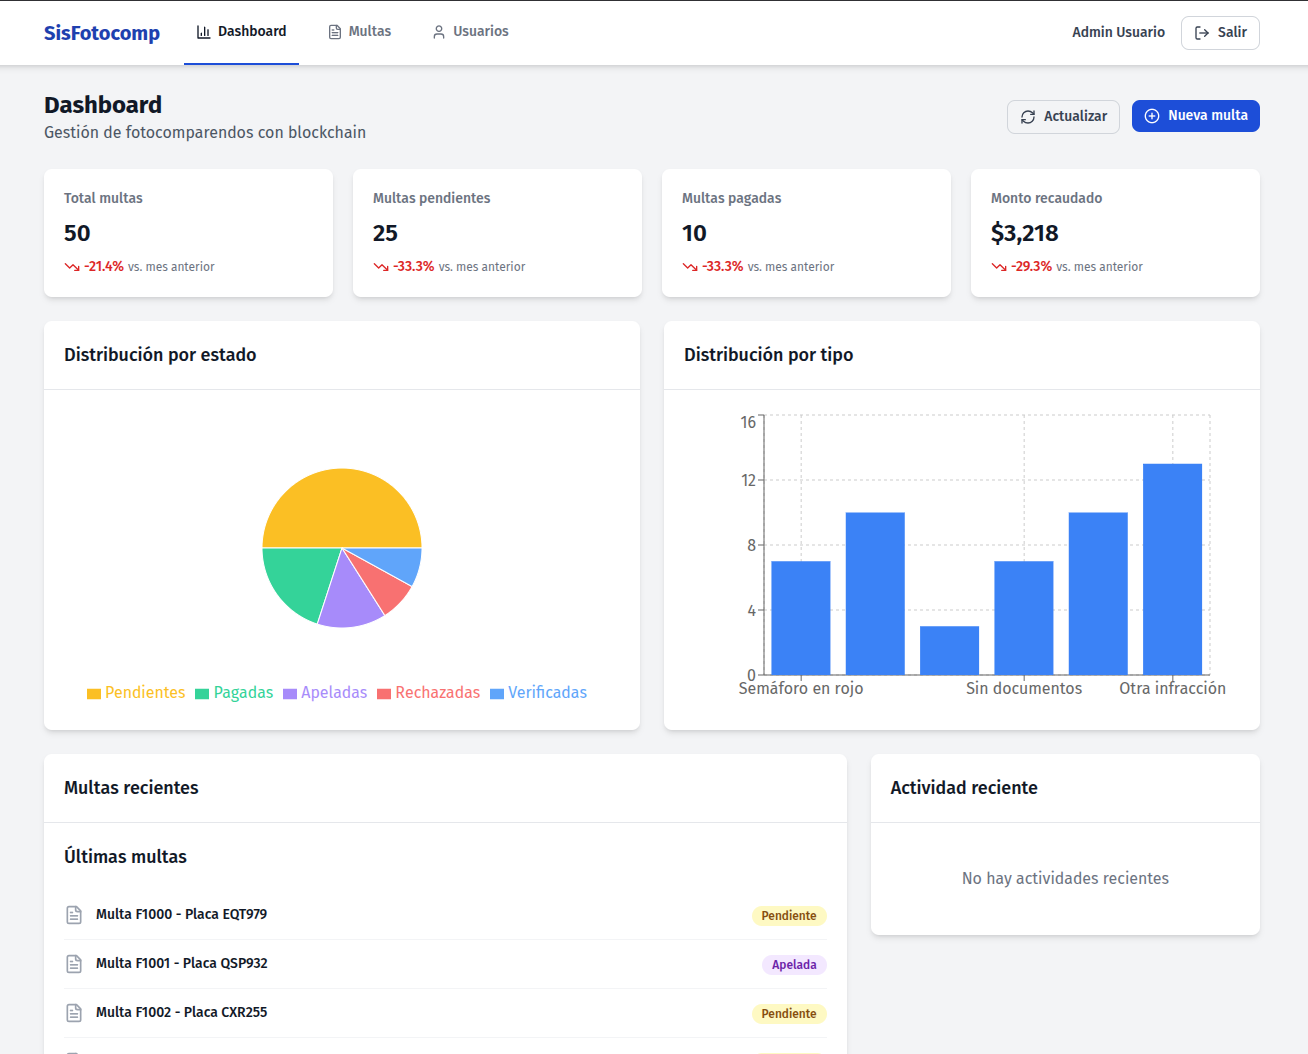
\includegraphics[width=0.8\textwidth]{Images/UI3.png}
    \caption{Dashboard del agente de tránsito.}
    \label{fig:dashboard_agente}
\end{figure}
+En la Figura~\ref{fig:dashboard_agente} se presenta el tablero principal que resume las métricas de gestión de multas para el agente de tránsito.
\begin{figure}[htbp]
    \centering
    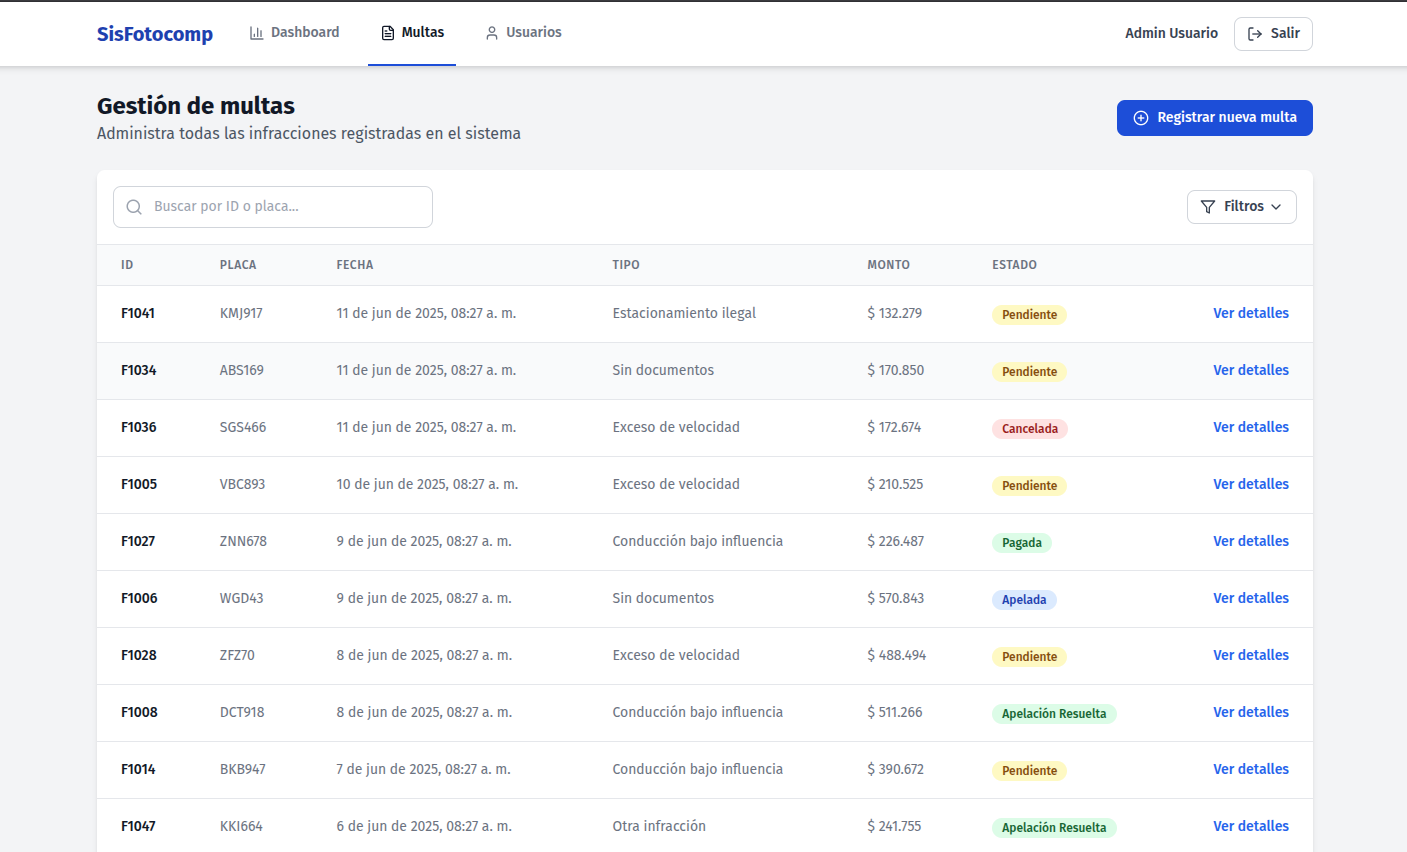
\includegraphics[width=0.8\textwidth]{Images/UI4.png}
    \caption{Pantalla de consulta del estado de multa.}
    \label{fig:consulta_estado_multa}
\end{figure}
+La Figura~\ref{fig:consulta_estado_multa} ilustra la consulta rápida del estado de una multa, facilitando el seguimiento por parte del agente.
\begin{figure}[htbp]
    \centering
    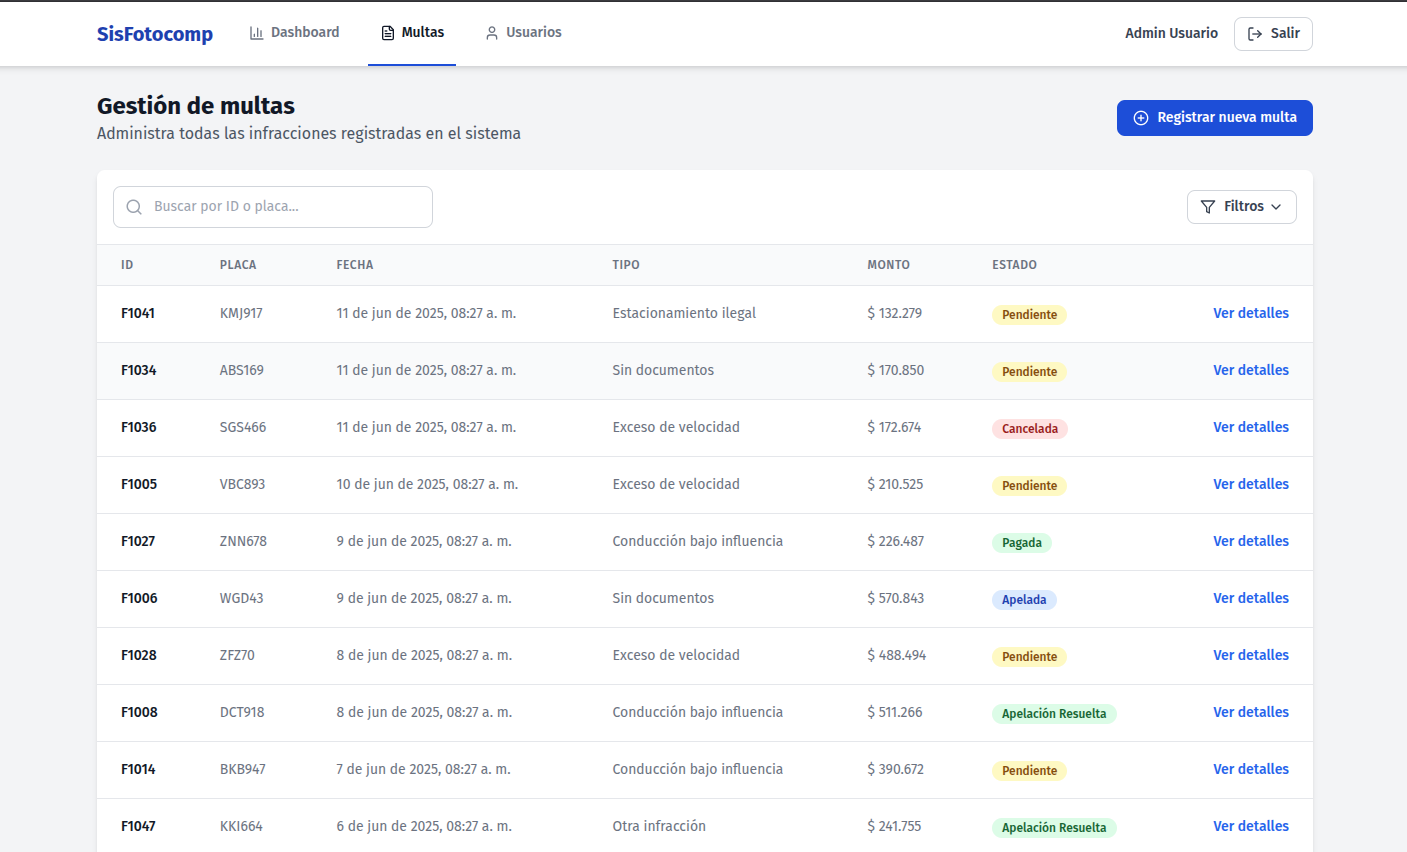
\includegraphics[width=0.8\textwidth]{Images/UI4.png}
    \caption{Pantalla de consulta de detalle de multa.}
    \label{fig:consulta_detalle_multa}
\end{figure}
+En la Figura~\ref{fig:consulta_detalle_multa} se muestra el detalle completo de una multa específica, incluida la evidencia asociada.
\paragraph{Vista Propietario de Vehiculo}
\begin{figure}[htbp]
    \centering
    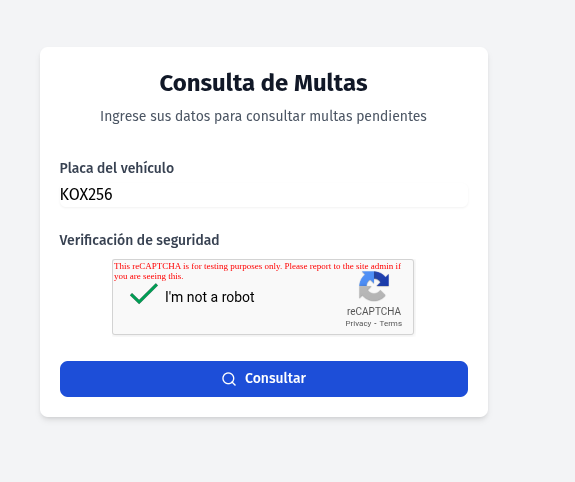
\includegraphics[width=0.8\textwidth]{Images/UI5.png}
    \caption{Pantalla de consulta de multas para propietarios de vehículos.}
    \label{fig:consulta_multas_propietario}
\end{figure}
+Por último, la Figura~\ref{fig:consulta_multas_propietario} exhibe la vista que permite al propietario del vehículo revisar todas sus multas pendientes o en proceso. 